\documentclass[12pt]{article}
\usepackage[a4paper,left=2cm, right=2cm, top=2cm, bottom=2cm]{geometry}
\usepackage{amssymb}
\usepackage{amsmath,mathtools}
\usepackage{relsize}
\usepackage{epsfig,graphicx}
\usepackage{color}
\usepackage{xcolor}
\usepackage{tikz}
% \usepackage{subfigure}
\usepackage{hyperref}
\usepackage{algorithm}
\usepackage{algorithmic}
\usepackage{cite}
\usepackage{amsfonts}
\usepackage{textcomp}
\usepackage{xcolor}
\usepackage{multirow}
\usepackage{authblk}
\usepackage{subcaption}

\begin{document}

% \def\BibTeX{{\rm B\kern-.05em{\sc i\kern-.025em b}\kern-.08em
%  T\kern-.1667em\lower.7ex\hbox{E}\kern-.125emX}}

\title{Route Optimization For Waste Collection\\}
\date{}
\author[1]{Marut Priyadarshi}
\author[2]{Meet Maratha}
\author[3]{Mohammad Anish}
\author[4]{Vaibhav Kumar}
\affil[1]{Department of Data Science Engineering, IISER Bhopal}
\affil[2]{Department of Data Science Engineering, IISER Bhopal}
\affil[3]{Department of Physics, IISER Bhopal}
\affil[4]{Department of Data Science Engineering, IISER Bhopal}

\maketitle

\section{Introduction}

Solid Waste Management (SWM) is considered one of the critical drivers of urban environmental management systems \cite{hoornweg2012waste}.It is generally an exercise to collect the combined waste from households, agricultural, industrial, commercial activity, institutional, and miscellaneous, generated from the living community \cite{GUPTA2015206}. India is one of the least urbanized countries in the world, yet urban India produces about 42.0 million tons of municipal solid waste annually, i.e., 1.15 lakh metric tons per day (TPD) \cite{SHARMA2021293,GUPTA2015206}. These figures are bound to increase in the future, as cities are witnessing extreme demographic transfers, immigration, population growth, and consumption rate, which are the key driving factors for the increase in urban waste. This has become one of the most urgent concerns for local agencies in India. During the last decade, the government has launched various programs e.g., Clean India Mission, Smart Cities, Amruth Cities, and Digital India to improve living standards. Waste management is one of the core infrastructure elements of these missions, which requires empirically driven conclusions to address the SWM related challenges \cite{CHEELA2021419}. 

Solid waste collection is the most integral activity of SWM. However, the waste collection in India is very unorganized, primarily due to resource constraints and poor planning of available resource \cite{somani2021integrated,GUPTA2015206}. Collection vehicle route planning (VRP) is the major resource component of a waste collection system, whose planning is often not driven by analytics, resulting in poor collection efficiency \cite{akbarpour2021innovative}. Similar scenarios have been reported by in almost every city in developing countries \cite{GUPTA2015206}. VRP requires modeling many components such as path planning, consideration of available resources, spatiotemporal demand patterns, and real-time dynamics of waste volume at collection points and trucks. A plethora of literature addresses subsets of these components in solution development. However, a holistic waste collection system that considers them simultaneously for any region has not been reported in the literature \cite{han2015waste}. Hence, the onground implementation of the present approaches are still very limited. This significantly impacts the operation costs and, eventually, the environment \cite{apaydin2007route}. Moreover, the components and their interrelationships are very complex for the resource-constrained societies, and therefore pose new challenges that require the researchers' urgent attention.

To address the challenges stated above, we propose a waste collection framework for cities, with the objective to find the optimal routes for the available vehicle paths while considering the dynamic variations in the waste information at collection points and also that of the vehicles. We also discuss the influence of available resources in covering the collection bins, whose dynamic information drives the best path. Finding the best path is formulated as an optimization problem and solved using linear programming. The approach has an advantage over other traditional path planning approaches due to the considerations of field-based activities in the model. Further, the study  focuses on resource-constrained societies resulting in a decision making tool that can be scaled and applied universally. Moreover, being dynamic in nature our model can calculate optimal routes, replicating the real-time scenarios. Hence, can help fill the gap a between theory and on ground implementation. The paper has following major contributions:

\begin{itemize}
\item Analysis of truck availability in study regions on waste collection, to demonstrate the total coverage.
\item Consideration of quantitatively simulated dynamic waste levels for truck and
collection bins for realistic outcomes.
\item Detailed sensitivity analysis of various parameters affecting selection of the best path.
\end{itemize}


\section{Related Studies}

A lot of work has been done in different aspects of waste collection, such as the costs, route optimization, smart bins, segregation, landfill and collection depot optimal locations. But, by far, the most common topic of work in this area has been Vehicle Routing Problem (VRP) in recent years. These works mostly address the problem of route optimization of collection vehicles for various cases such as landfill and collection sites allocation to minimize distance traveled by collection vehicles \cite{kulcar1996optimizing,rathore2020location,barzehkar2019landfill}, collection point clustering to increase collection efficiency \cite{al2021optimization} and calculating the optimal route with a fixed set of collection nodes and landfill/depot locations \cite{karadimas2008routing, amal2018sga, asefi2019mathematical,de2007decision, hannan2020waste,akhtar2017backtracking}. The mathematical calculations of the VRP have been solved through various preexisting route optimizers  \cite{karadimas2008routing,amal2018sga, malakahmad2014solid}, or by formulating the problem as single or multi-objective functions \cite{hannan2020waste,de2007decision}. The biggest drawbacks of these models is that they are predominantly static and calculate the optimal routes once for a set of collection points. Some studies have modeled the some dynamic aspects in the  routing such as dynamic routes and its impact on fuel consumption\cite{hannan2020waste},smart bins to track waste \cite{akhtar2017backtracking,lozano2018smart,baldo2021multi}. However, they lack the integration of real world aspects such as changes in routes based on the status of other vehicles etc., hence, are often not implemented in decision making system\cite{hannan2020waste}. Further, most of such works are developed for the cities of developed nations which are not resource constrained, and have less challenges as compared to cities of developing nations.\\
Waste collection in resource constrained societies comes with the additional challenge of having to allocate insufficient resources to meet the demand. There are many studies that have been implemented on the cities of developing nature  that focus on this aspect of waste collection. \cite{chaudhary2019gis} and \cite{sk2020optimal} utilized Geographic Information Systems (GIS) to calculate optimal waste collection routes in the city of Allahabad and Durgapur in India respectively. Theese studies, however, didnt consider any dynamic considerations.\cite{ogwueleke2009route} and \cite{malakahmad2014solid} focused on route optimization in the cities of Onitsha, Ipoh , and Malaysia respectively.  \cite{rathore2020location} focused on optimal node allocation to maximize the waste collection in the city of Bilaspur, India.  These works, however, do not consider any real time data to calculate the optimal routes. 
There are a some excellent reviews by \cite{belien2014municipal,sulemana2018optimal,abdallah2020artificial} that a reader can refer to study the works related to optimization of waste collection and management systems. 


% In one paper \cite{kulcar1996optimizing}, the author focuses on the best location for the construction of a landfill that would result in the shortest collection routes when linked with the currently existing routes and depots. The paper also compares the running costs of different modes of waste transport, such as trains, ships and by road. It was useful in providing a picture of the costs associated with the system, it didn't focus on optimizing the routes that the waste collection was done. Moreover, it was set in Brussels, a highly developed city. In a similar vein, Rathore et al. \cite{rathore2020location} focuses on formulating a mathematical model for finding the optimal places to allocate bins in the Indian city of Bilaspur. While it aims towards the similar goal of waste collection optimization, furthermore in a developing country, the method is different from our intended goal.

% Many papers utilize pre-existing solvers or software to compute the optimized routes and use the results to compare them to other algorithms or observe the effects the optimized routes bring to the current system. In the case of one paper \cite{karadimas2008routing}, the sole focus of the paper is on route optimization. However, it only applies ant colony system and the route optimizer for the software ArcGIS Network Analyst to get the optimal route for non-real time data and compares the efficiencies of the two methods. Moreover it focuses on Athens, another developed city, and even then on only one prefecture of it. Similarly, Chaudhary et al \cite{chaudhary2019gis} have utilized ArcGIS Network Analyst software to calculate optimal routes for waste collection, this time in the city of Allahabad. This lies closer to our goal of route optimization for more resource constrained societies and while it is an extensive application of optimization process utilizing the real-life data from the city, it still only utilizes a pre-existing algorithm along with fixed unchanging datapoints to calculate the collection routes, which our work seeks to expand upon. Another paper \cite{amal2018sga} uses the route optimization solver of GIS software ArcGIS (which itself utilizes Dijkstra algorthm) to calculate a pool of routes which, in turn, feeds the genetic algorithm to iteratively arrive at the optimal routes for the waste collection vehicles.

% In their paper, Simonetto and Borenstein \cite{de2007decision}, used linear programming to formulate a function for route optimization via minimization of cost coupled with a heuristic developed by Renaud and Boctor \cite{renaud2002sweep} in order to bring down the computation time (at that time) to reasonable levels. Similarly, in this paper \cite{hannan2020waste}, the authors have used linear programming combined with smart bins to find optimal waste collection routes that remove the inefficiency that is associated with formulating a route that visits all nodes, regardless of its fill status. However, as it was a paper focused on the algorithmic part of the problem, they used purely simulated data, void of any real world analogue and only factored in the euclidian distances between the nodes. Asefi et al \cite{asefi2019mathematical} uses a mixed-integer linear programming model to minimize costs and uses two different meta heuristic approaches to deal with the non-deterministic polynomial-time hardness of the waste collection problem. This model is then applied to a case study in the city of Tehran, Iran. 

% In other papers utilizing smart bins, Akhtar \cite{akhtar2017backtracking} utilizes new population based meta heuristic backtracking search optimization, developed by Civicioglu \cite{civicioglu2013backtracking}, to calculate optimal routes for collection vehicles. Its main feature is its simplicity as it has only one control parameter. It is also a highly theoretical work and focuses mainly on the mathematical aspects of the problem and not its real-life application. Al-Refaie et al \cite{al2021optimization} takes a different approach and focuses instead on distributing the collection points into optimal clusters so that the collection efficiency of the vehicles can be maximized.

% Papers like Lozano et al \cite{lozano2018smart} and later Baldo et al \cite{baldo2021multi}, Vishnu et al \cite{vishnu2021iot} use smart bins, but the focus of these papers are the smart bins themselves, their engineering aspect and case studies involving them, along with constructing a system centered around technology which automates a lot of the tasks involved in the whole process of waste collection and management. The optimization part is left to pre-existing solving algorithms.

% Smart bins have also been discussed in a more theoretical aspect, utilizing IoT technology in other studies such as Abdullah et al \cite{abdullah2018iot}, Ali et al \cite{ali2020iot}, Al-Masri et al \cite{al2018serverless} and Chaudhari and Bhole \cite{chaudhari2018solid}. They have touched upon smart bins as parts of a sustainable smart city architecture and different ways that they may be utilized, along with supporting subsystems. It should be noted that the above-cited literature is in no way an exhaustive list of literature utilizing IoT or smart bins, and merely provides a general idea of the works using it.



\section{Problem Definition and Mathematical Formulation}


\subsection{Problem Definition}
The waste vehicle routing problem in dynamic settings is implemented using agent-based modeling approach. A collection vehicle is an individual goal driven agent that implements an optimization module to achieve its goal of routing on a good path. A path is calculated by minimizing the distance traveled and maximizing the waste collected while considering various real-time considerations. We have considered an Indian city to demonstrate its outcomes. To implement the model we have divided the study area in various regions. The region consists of smart collection bins used to collect waste and generally caters to a large area. These bins as nodes are assumed to be located on a road network made from edges and nodes. We simulated temporally varying waste values (0-100\%) for each of these bins; we call them” smart bins”. The simulation helped us overcome the requirement of physical sensor placement at these locations. We incorporated the inputs of stakeholder agency in the simulation purpose to keep the simulation values closer to the actual scenarios.\\
\\
\textbf {Input}\\
\textit {Agent:} Waste collection vehicle.\\
\textit {Agents attributes:} Waste fill percentage, distance traveled.  \\
\textit {Environment:} Road network, bins, depot.  \\
\textit {Environment attributes:} Waste percentage of bins, route length, distance between each node.\\
\textbf{Outcome}\\
Best path for each agent\\

An agent is initially assigned to a specific region, and it only collects waste from bins from the assigned region through the calculated optimal route. The” route” in our problem corresponds to path of the agent covering these bins and finishing its trip at a fixed depot. A path is made up of non-directional edges, and two or more edges make an “arc”. To make the implementation realistic we have applied limits on the total waste that the agents can collect. When the waste from a bin is collected by an agent the waste value of the vehicle is updated, and the numerical values of the distances are normalized to the same scale as the waste values to avoid any execution bias.\\
The model is executed after a specific time interval by considering updated bins waste values, vehicle waste fill status, and vehicle location to generate a route. The route is updated after every fixed time interval. A priority is being given to a bin based on the distance to that bin from the agents current location and the waste value of bin. This means that a bin with the greater waste value is assigned a higher priority for the same distance value. When the waste from a bin is collected by an agent the waste fill percentage of the vehicle is updated. 
The execution for any agent terminates when either a run is complete, or the vehicle is full. The ”run” in our problem signifies the process of agents reaching the depot through calculated routes in various time intervals. As the agents execute in parallel, if an agent, in one time interval fails to visit a does not visit a node because being full, other agent can cater the bin. We also considered the case when bin waste values could update even when the vehicle is moving on an edge and hasn't reached the next node. For such scenarios the model assumes that the vehicle has completed the current edge and considers the next node as the starting point in the next time interval. 

\begin{figure}[H]
    \centering
    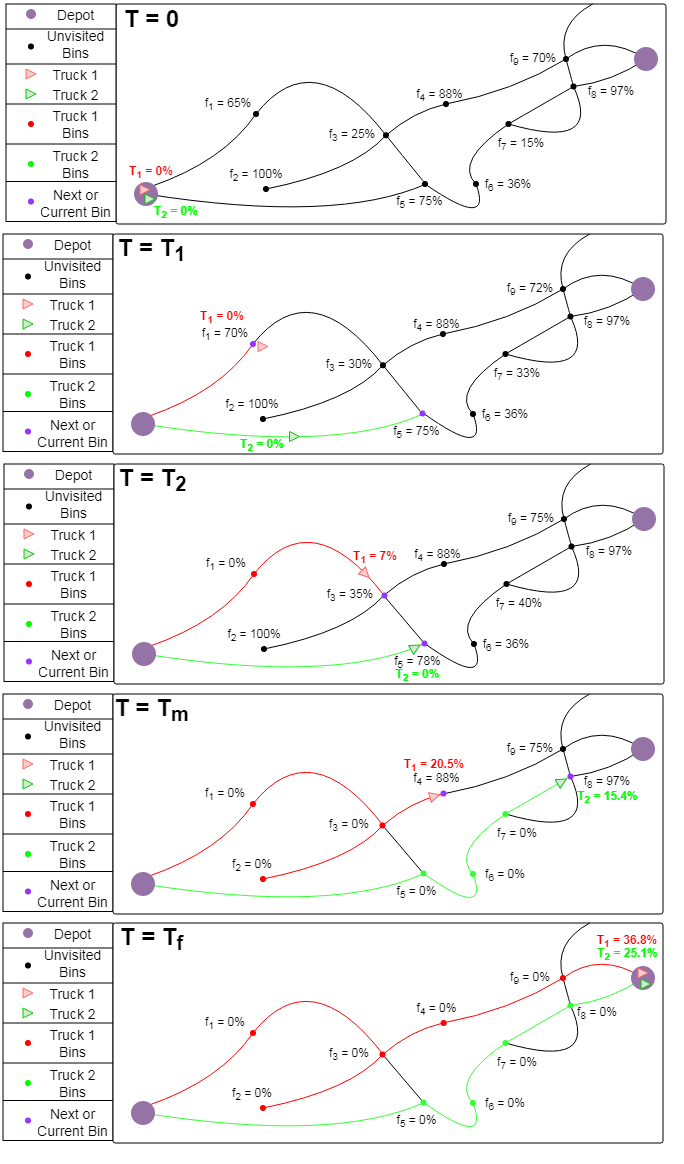
\includegraphics[scale=0.6]{ExplainationFigure.png}
    \caption{General representation of the process}\label{fige}
\end{figure}

Figure \ref{fige} depicts the discussed problem definition. Figure 1a depicts the starting state of the two agents $T=0$ at depot, and the percentage fill values for various bins (b1..b7). The fill percentage of agents are also shown. Figure 1b-1d illustrate the further time intervals ($T=T_1,T_2,T_m$) and the dynamic changes in the movement of truck and their fill percentage, updates in the bin fill percentage, and updated routes after each time intervals. It can be noted that truck1 goes to depot at  $T=m$ as its fill percentage becomes 100. The routes at that time is generated to move the truck on the shortest path to depot. Figure 1e depicts the last state at time interval $T=T_f$ when the agents finally return to the depot node at the final time $T=T_f$.

Four different execution scenarios are demonstrated. The first scenario restricts the available resources, which in our case is the collection vehicles. The second case runs the model without any restriction on available resources and demonstrates the impact of available resources on waste collection, bins covered and distance travelled for each region and accumulated at city scale. Lastly we emphasize the importance of dynamic consideration by comparing the outcome of dynamic model with the static model.

\subsection {Mathematical Formulation}

The objective of the model is to maximize the waste collected while minimizing the total distance travelled by the vehicles. We formulate the model as a mixed integer linear programming problem and solved it using Gurobi optimizer \cite{gurobi} in polynomial time. Such solvers can solve problems with realistic instance sizes, which was in our case.

In our problem, our two main objectives are:
\begin{itemize}
    \item Minimize the distance travelled by the collection vehicles
    \item Maximize the waste collected through the collection run
\end{itemize}

Table1 defines all the variables used in the mathematical formulation.
\begin{table}[H]\label{variables}
	\centering
	\caption{The description of variables}
	\begin{tabular*}{486pt}[H]{|c|c|}
		\hline \hspace{40pt} Variables \hspace{40pt} & \hspace{130pt} Description \hspace{130pt} \\
		\hline $i, j \in D$ & Node i and Node j respectively.\\
		\hline $N$ & Nodes for a particular truck excluding depot.\\
		\hline $D$ & Nodes for a particular truck including depot.\\
		\hline \multirow{2}{*}{$A$} & Set of all the arcs formed from a\\
		&  node i to a node j for $\forall i,j \in$ V.\\
		\hline \multirow{2}{*}{$C_{ij}\in \mathbb{R}^+$} & Distance cost from a node i\\
		& to a node j for a truck.\\
		\hline \multirow{2}{*}{$X_{ij} \in \{0, 1\}$} & It is a binary variable that is 1 if a truck is\\
		& travelling between the node i and node j.\\  
		\hline \multirow{2}{*}{$Y_{i} \in \{0, 1\}$} & It is a binary variable that is 1 if a truck is \\
		& visiting node i.\\
		\hline \multirow{2}{*}{$u_{i}  \in [0, 100 -P_{t}] $} & The percentage fill of the truck at node i \\
		& following given path, for a specific time slice.\\
		\hline \multirow{2}{*}{$st \in D$} & The starting node of a truck in a\\
		& new time slice.\\
		\hline \multirow{2}{*}{$w_{1} \in [0.0, 1.0]$} & The weight assigned to the distance \\
		& objective of the objective function\\
		\hline \multirow{2}{*}{$w_{2} \in [0.0, 1.0]$} & The weight assigned to the waste amount \\
		& objective of the objective function\\
		\hline \multirow{1}{*}{$f_{i} \in [0.0, 1.0]$} & The fill ratio of bin at node i.\\
		\hline \multirow{2}{*}{$BT \in \mathbb{R}^+$} & The conversion factor for fill \\
		& of smart bin to fill of truck.\\
		\hline \multirow{1}{*}{$P_{t} \in [0.0, 100.0]$} & Cumulative fill percentage of truck at a time slice t.\\
		\hline
	\end{tabular*}
\end{table} 

The objective function is formulated as:

\begin{equation}\label{eq1}
    Obj(minimize)=\sum_{i,j \in A} w_1 X_{ij} C_{ij} - w_2 Y_i f_i * BT
\end{equation}

Here, $X_{ij}$ is a binary variable that can only take the values 0 or 1, based on the fact whether a truck took a route from i to j or not. $C_{ij}$ is the cost, or the distance travelled when moving from i to j. $Y_{i}$ is another binary variable that indicates if waste from node i has been collected or not. $BT$ is the conversion factor of how much would the waste from a node would fill up a truck collecting it. $f_i$ represents the fill ratio (the percentage of how full the bin is) of the bin, its value being between 0 and 1. 0 meaning it is empty and 1 meaning it is full. The variables $w_1$ and $w_2$ are the weights associated with distance travelled and waste collected, respectively.

The weights $w_1$ and $w_2$ sum up to one as shown by Equation (2). following constraint applies:

\begin{equation}\label{eq1.5}
    \sum_{n\in \{1,2\}} w_n = 1
\end{equation}

Later we have discussed a detailed sensitivity analysis of the weight selection on objective function. 

The subscript 'st' denotes the starting node at the start of each time interval. The constraint (3) 
\begin{equation}\label{eq2}
    \sum_{j\in N}X_{st,j}=1 ; \forall st \in D ; j \in N
\end{equation}
\begin{equation}\label{eq3}
    \sum_{j\in N}X_{j,0}=1 ; \forall j \in N
\end{equation}
Node 0 is assigned to be the depot, the start and the end point of every collection run. Eq (\ref{eq2}) and Eq (\ref{eq3}) ensure the looping of the route, with the added caveat that since the calculations are made multiple times per run (called time slices) as new data is obtained, the value of the starting node for each subsequent time slice, after the initial one, changes. Therefore, these new starting nodes have to also be taken into consideration.
\begin{equation}\label{eq4}
    \sum_{i\in N}\sum_{j\in D } X_{ji}=1 ; \forall i,j \in A ; j\ne i
\end{equation}
\begin{equation}\label{eq5}
    \sum_{i\in N}\sum_{j\in D } X_{ij}=1 ; \forall i,j \in A ; j\ne i
\end{equation}
Eq \eqref{eq4} and Eq \eqref{eq5} specify that the nodes that are already visited by the truck in a collection run are not considered again for for further calculations, or in simpler terms, a node that has already been visited is not visited again in the same run.

The variable $u_i$ is a temporary variable that resets to zero at the beginning of each time slice. It represents the percent the the truck is full for each separate calculation. Variable $P_t$ is the variable that stores all the cumulative progress of how full the truck is, in percent, over all the previous and subsequent time slice.

If:
$$ X_{ij}=1$$
then:
\begin{equation}\label{eq7}
    u_i+f_j*BT =u_j ; \forall i,j \in A 
\end{equation}
for: 
$$ i,j\ne 0$$
$$ i,j \ne st $$
This constraint (Eq \eqref{eq7}) ensures that if a truck goes on an arc (an arc being a small portion of the entire collection route) from two consecutive nodes, node i to node j, the amount of waste is continuous, that is, the waste in the truck at node j is the sum of the waste at node i and the waste collected in the route i to j. The value of the waste inside the truck is updated at node j so that there is no discrepancy in the case when a new path has to be calculated with new data.
\begin{equation}\label{eq8}
    u_i\ge f_i*BT
\end{equation}
$$  \forall i\in N$$
Eq \eqref{eq8} ensures that the amount of waste in a truck after reaching a node must be greater than or equal to the waste it had before that. This makes sure that the truck is actually collecting the waste from that node and not just passing it.
% Added this equation
\begin{equation}\label{eqY}
	\sum_{i\in N}Y_i f_i* BT\le100-P_t
\end{equation}
Eq \eqref{eqY} ensures that the truck will not collect waste from a node if collecting from that node makes the truck exceed its maximum capacity. Therefore, for the sake of maximizing waste collected, such nodes will not be taken into consideration for further time slices.
\begin{equation}\label{eq12}
    u_i\le 100 - P_t
\end{equation}
$$\forall i \in N $$
This constraint in Eq \eqref{eq12} ensures that for a single time slice in the collection run, the value of how full the truck is does not exceed its capacity. Since $P_t$ stores the cumulative fill percentages of the truck, in any subsequent and previous time slices, the fill percent of the truck should not exceed the sum of the previous fill percentage and the percent filled in the current calculation. 

With this, we have formulated our problem and now we can move on to implementing and calculating the solution for our problem

\section{Case Studies and Empirical Results}

\subsection{Data Preparation}

To prove the effectiveness of the model, we empirically tested the model for the city of Chandigarh in India. The city is located by the foothills of the Shivalik range of the Himalayas in northwest India. It covers an area of approximately 114 km$^2$. It borders the states of Punjab and Haryana. The city is known for being the first planned city of India. The city also has various scattered unplanned built-up patches such as Burail, Nayagaon. The mixed built-up typology was suitable to test the methodology. Hence, the city was found suitable to test the methodology. We generated various waste collection points (location of smart bins) for the city. A total of 300 points were generated randomly using Geographic Information System (GIS) functionalities, with the constraint that the point should fall on the road networks. The road network was extracted from Open Street Map (OSM) database. OpenStreetMap API was then used to calculate the distance between all nodes, and generate a distance matrix which was used in the optimization process. We applied K-Means clustering algorithm to cluster these points in a fixed set of clusters (see Figure 1). In this paper we have selected total clusters to be three. The number can be updated based on user requirements. After clustering, region1, region2 and region3 had 95, 111 and 94 points, respectively. The clusters were considered as three regions for which vehicles had to be allocated. To replicate the actual field activities we have considered that a vehicles starts and ends its route at the depot (see Figure) \ref{figm})


\begin{figure}[H]
    \centering
    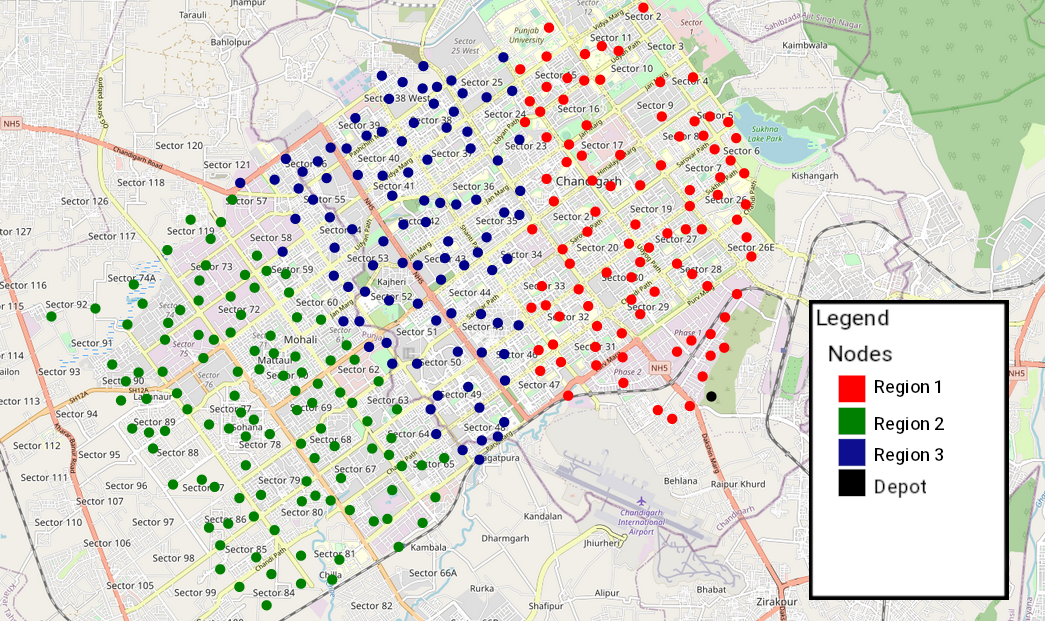
\includegraphics[scale=0.4]{Nodes.png}
    \caption{The selected nodes and their clusters}\label{figm}
\end{figure}

\subsection{Execution case studies}
Experiments were carried out on a AMD A6-9220 processor which runs at 2.5GHz and utilizes 8 GB RAM. The model was implemented in Python 3.10.5 and solved with Gurobi optimizer version Gurobi 9.5.1. A total of four scenarios were implemented and the minimum and maximum solving time was around 67.0618 s having total variable count: 7041 and total constraint count: 7075 for the maximum case.

As per Dengel et al \cite{degel2015time}, one of the most common approaches to handle multi-criteria decision problems is the weighted sum approach. In this approach, the objectives are aggregated prior to the optimization by assigning weights to the objective functions. The weights are based on the decision makers preference in order to model the importance of the goal, which in our case is to find minimum path route while maximizing the collected waste. 

The suggestion of the decision makers (Municipal Corporation Chandigarh) was to provide equal preference to find minimum distance routes and maximizing the waste collection. hence, we assigned  $w_1$ and $w_2$ to be 0.5 to execute the scenarios. This means that our optimization model gives equal importance to minimizing the distance and maximizing the waste collected. To highlight the important of weights a detailed sensitivity analysis of weights on outcomes is discussed later in a subsection.
The maximum available number of collection vehicles (mv) was considered to be 7, and was considered same for all the regions. The values are selected based on the input of the decision makers. The maximum capacity of a truck (TC) was considered as 1000 Kg, and the maximum capacity of a smart bin (BC) was considered as 100 Kg.

\subsubsection*{Case 1: Restriction on Resources}
To highlight the importance of strategical usage of available resources in resource constraint societies, we applied restrictions on the available collection vehicles. The vehicle values were varied from one to six and the impact on total distance travelled, total waste collected, and total nodes covered was studied for each region, and  eventually for the city. The routes were calculated while considering the temporal dynamics of bin and waste level, truck positions in varying time-steps. Table \ref{tab1} illustrates the cumulative values for the distance and wastes outcomes for all the trucks in each region.
\begin{table}[H]
    \centering
    \caption{Data for the real-time restricted case} \label{tab1}
    \vspace*{0.3cm}
    % Following are the changes
    \hspace*{-1cm}
    \begin{tabular}{|c|c|c|c|c|c|c|}
        \hline \multirow{2}{*}{Case} & \multicolumn{2}{c|}{Region 1} & \multicolumn{2}{c|}{Region 2} & \multicolumn{2}{c|}{Region 3}\\
        \cline{2-7}& Waste (Kg)  & Distance (Km) & Waste (Kg) & Distance (Km) & Waste (Kg) & Distance (Km)\\ 
        \hline \textit{1 Truck} & 999.89 & 39.79 & 997.36 & 63.11 & 999.94 & 59.22 \\
        \hline \textit{2 Trucks} & 1992.68& 99.58 & 1994.29 & 129.37 & 1984.23& 119.51 \\
        \hline \textit{3 Trucks} & 2989.61 & 142.05 & 2997.77 & 195.04 & 2979.87 & 180.71 \\
        \hline \textit{4 Trucks} & 3989.43 & 208.59 & 3986.17 & 279.63 & 3977.46 & 241.80 \\
        \hline \textit{5 Trucks} & 4961.06 & 321.16 & 4966.69 & 345.68 & 4964.88 & 322.97 \\
        \hline \textit{6 Trucks} & 5282.82 & 362.89 & 5959.62 & 433.19 & 5179.85 & 373.26 \\
        \hline
    \end{tabular}
\end{table}

A significant impact of available trucks on collected waste can be observed. Further, the increase in waste collected for different number of trucks per region varied linearly for each region to the total distance traveled by all the trucks (Figure \ref{figz}). The increase in distance and collected waste is a direct result of having more trucks running at the same time. For region1 and region3, a sharp drop in the waste collected was observed after five trucks. Which means almost all the smart bins for these regions was catered by these trucks. On the other hand region2 still required more resources to cater the demand. This is more evident by Table \ref{tab3}, which details the case of 6 trucks per region to determine whether it is sufficient to satisfy the waste collection demand of regions and the city. It can be observed all bins for regions 1 and 3 were covered by utilizing 6 trucks, while only 85\% of the nodes for region2 were covered by the six trucks. This is primarily because the value of waste for the bins in this regions was higher due to region2 having more nodes than region1 and region3.

\begin{figure}[H]
    \centering
    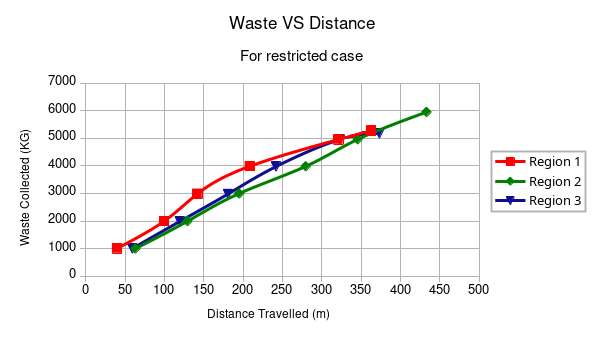
\includegraphics[scale=0.6]{distance_VS_garbage_restricted.png}
    \caption{Distance traveled vs waste collected}\label{figz}
\end{figure}
\begin{figure}[H]
    \centering
    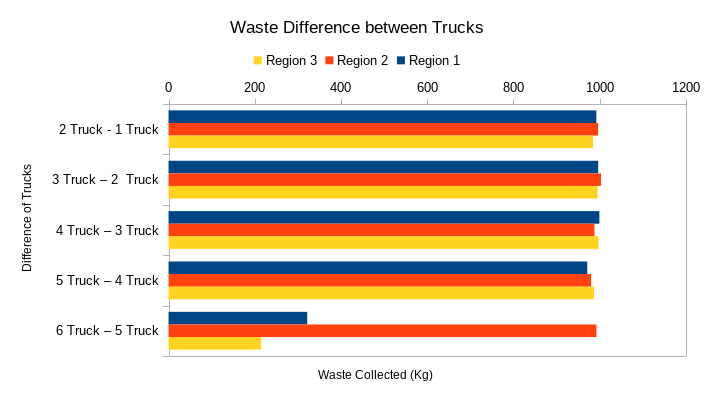
\includegraphics[scale=0.6]{Waste Difference Between Trucks.png}
    \caption{Difference in waste between cases}\label{figd1}
\end{figure}
\begin{figure}[H]
    \centering
    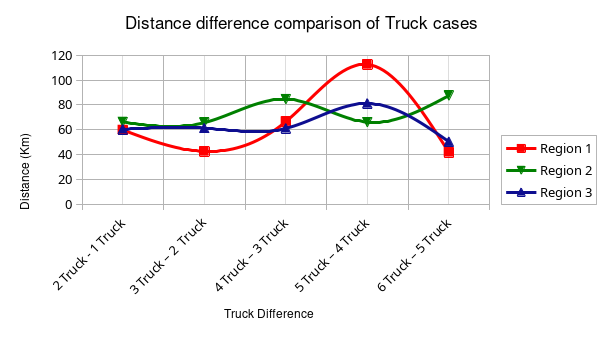
\includegraphics[scale=0.6]{Distance Difference Between Trucks Scatterplot.png}
    \caption{Difference in distance between cases}\label{figd2}
\end{figure}
\textcolor{red}{As observed in Figure \ref{figd1}, the difference of the increase of waste collected for the cases of different number of trucks per region is linear, that is, the difference remains more or less the same. This also appears to be true for the case of distance (Figure \ref{figd2}), which has slight deviations from a completely linear trend, but the deviations occur for both sides of the graph, making the deviations effectively inconsequential.}
\begin{table}[H]
    \centering
    \caption{ Data for 6 trucks per region} \label{tab2}
    \vspace*{0.3cm}
    % Changed Values
    \begin{tabular}{|c|c|c|c|c|c|}
        \hline Region & Truck & Waste (Kg) & Distance (Km) & Waste/Distance & Percent collected \\
        \hline \multirow{4}{*}{Region 1} & Truck 1 & 999.07& 38.53 & 25.93 &14.7368\% \\
        \cline{2-6}& Truck 2 & 990.67 & 47.20 & 20.99 & 13.6842\%\\        
        \cline{2-6}& Truck 3 & 994.66 & 43.57 & 22.83 & 15.7895\%\\        
        \cline{2-6}& Truck 4 & 998.21 & 72.55 & 13.76 & 20.0000\%\\      
        \cline{2-6}& Truck 5 & 977.66 & 121.86 & 8.02 & 24.2105\%\\      
        \cline{2-6}& Truck 6 & 322.56 & 39.19 & 8.23 & 11.5789\%\\
        \hline & & & &\textbf{Total:} &\textbf{100\%}\\
        \hline \multirow{4}{*}{Region 2} & Truck 1 & 999.71 & 62.64 & 15.96 & 12.6126\% \\
        \cline{2-6}& Truck 2 & 993.32 & 71.67 & 13.86 & 12.6126\%\\        
        \cline{2-6}& Truck 3 & 985.38 & 56.82 & 17.34 & 14.4144\%\\        
        \cline{2-6}& Truck 4 & 991.47 & 78.51 & 12.63 & 13.5135\%\\        
        \cline{2-6}& Truck 5 & 990.43 & 64.48 & 15.36 & 13.5135\%\\        
        \cline{2-6}& Truck 6 & 999.31 & 99.06 & 10.09 & 18.9189\%\\
        \hline & & & &\textbf{Total:} &\textbf{85.5856\%}\\     
        \hline \multirow{4}{*}{Region 3} & Truck 1 & 999.68 & 48.07 & 20.80 & 15.9574\% \\
        \cline{2-6}& Truck 2 & 998.71 & 55.13 & 18.12 & 15.9574\%\\        
        \cline{2-6}& Truck 3 & 991.22 & 50.32 & 19.70 & 14.8936\%\\        
        \cline{2-6}& Truck 4 & 998.88 & 74.83 & 13.35 & 21.2766\%\\      
        \cline{2-6}& Truck 5 & 955.92 & 87.04 & 10.98 & 23.4043\%\\      
        \cline{2-6}& Truck 6 & 235.45 & 57.88 & 4.07 & 8.5106\%\\
        \hline & & & &\textbf{Total:} &\textbf{100\%}\\
        \hline      
    \end{tabular}
\end{table}

\subsubsection*{Case 2: Real-time, unrestricted}

Often the decision makers want to derive the requirement of resources that could cater to the whole demand. To achieve that, we relaxed the constraint on available resources to deduce the the total resource requirement for achieving 100\% bin visits, with high waste. In the previous case it was established that six trucks would cater to all the bins for region1 and region3. We extended the experiment for region2 by increasing the available trucks till we achieved 100\% bin coverage. It was observed that region2 was fully covered by seven trucks (see Table \ref{tab3}). Hence, given the existing bins, the city requirements can can be  fulfilled by 19 trucks (see Figure \ref{figc1}). Figure \ref{fig2} shows the calculated routes for each trucks of regions to depot.It can be noted that (see Figure \ref{figc2}) for region2, the rise in the percentage coverage of bins is less than the other two. This is primarily because region 2 is larger than region 1 and 3, and contains more nodes. This can be confirmed as the waste that is collected for equal number of trucks are similar to all regions. 


\begin{table}[H]
    \centering
    % Change the caption here
    \caption{ Data for unrestricted resources} \label{tab3}
    \vspace*{0.3cm}
    % Data changed here
    \begin{tabular}{|c|c|c|c|c|c|}
        \hline Region & Truck & Waste (Kg) & Distance (Km) & Waste/Distance & Percent collected \\
        \hline \multirow{4}{*}{Region 1} & Truck 1 & 999.07& 38.53 & 25.93 &14.7368\% \\
        \cline{2-6}& Truck 2 & 990.67 & 47.20 & 20.99 & 13.6842\%\\        
        \cline{2-6}& Truck 3 & 994.66 & 43.57 & 22.83 & 15.7895\%\\        
        \cline{2-6}& Truck 4 & 998.21 & 72.55 & 13.76 & 20.0000\%\\      
        \cline{2-6}& Truck 5 & 977.66 & 121.86 & 8.02 & 24.2105\%\\      
        \cline{2-6}& Truck 6 & 322.56 & 39.19 & 8.23 & 11.5789\%\\ 
        \hline &\textbf{Total:} &\textbf{5282.82} &\textbf{362.89} &- &\textbf{100\%}\\
        \hline \multirow{4}{*}{Region 2} & Truck 1 & 999.69 & 60.89 & 16.42 & 12.6126 \\
        \cline{2-6}& Truck 2 & 992.96 & 70.29 & 14.13 & 13.5135\%\\        
        \cline{2-6}& Truck 3 & 988.65 & 65.86 & 15.01 & 11.7117\%\\        
        \cline{2-6}& Truck 4 & 997.20 & 68.30 & 14.60 & 15.3153\%\\      
        \cline{2-6}& Truck 5 & 983.61 & 73.17 & 13.44 & 15.3153\%\\      
        \cline{2-6}& Truck 6 & 934.99 & 94.22 & 9.92 & 14.4144\%\\      
        \cline{2-6}& Truck 7 & 740.36 & 111.69 & 6.63 & 17.1171\%\\
        \hline &\textbf{Total:} &\textbf{6637.42} &\textbf{544.42} &- &\textbf{100\%}\\     
        \hline \multirow{4}{*}{Region 3} & Truck 1 & 999.68 & 48.07 & 20.80 & 15.9574\% \\
		\cline{2-6}& Truck 2 & 998.71 & 55.13 & 18.12 & 15.9574\%\\        
		\cline{2-6}& Truck 3 & 991.22 & 50.32 & 19.70 & 14.8936\%\\        
		\cline{2-6}& Truck 4 & 998.88 & 74.83 & 13.35 & 21.2766\%\\      
		\cline{2-6}& Truck 5 & 955.92 & 87.04 & 10.98 & 23.4043\%\\      
		\cline{2-6}& Truck 6 & 235.45 & 57.88 & 4.07 & 8.5106\%\\ 
        \hline &\textbf{Total:} &\textbf{5179.85} &\textbf{373.26 }&- &\textbf{100\%}\\
        \hline      
    \end{tabular}
\end{table}


% \begin{table}[H]
%     \centering
%     \caption{ Bins coverage in percent based on number of trucks per region} \label{tab4}
%     \vspace*{0.3cm}
%     \begin{tabular}{|c|c|c|c|c|c|}
%         \hline \multirow{2}{*}{Region} & \multicolumn{5}{c|}{Number of trucks}\\
%         \cline{2-6}& 1 Truck& 2 Truck& 3 Truck& 4 Truck& 5 Truck\\
%         \hline \textit{Region 1} & 11.5789\%& 41.0526\%& 60.0001\%& 69.4737\%& 98.9474\%\\
%         \hline \textit{Region 2} &9.9099\%&32.4324\%&52.2522\%&63.9636\%&72.9728\%\\
%         \hline \textit{Region 3} &11.7021\%&42.5532\%&58.5107\%&65.9574\%&99.9999\%\\
%         \hline
%     \end{tabular}
% \end{table}


\begin{figure}[H]
    \centering
    \begin{subfigure}{0.5\textwidth}
        \centering
        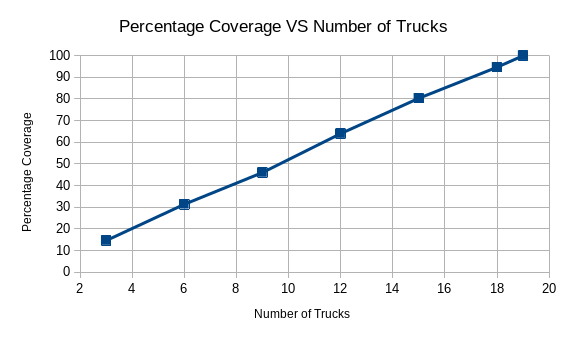
\includegraphics[width=\linewidth]{coverage_VS_number_of_trucks.png}
        \caption{For the entire city}\label{figc1}
    \end{subfigure}%
    \begin{subfigure}{0.5\textwidth}
        \centering
        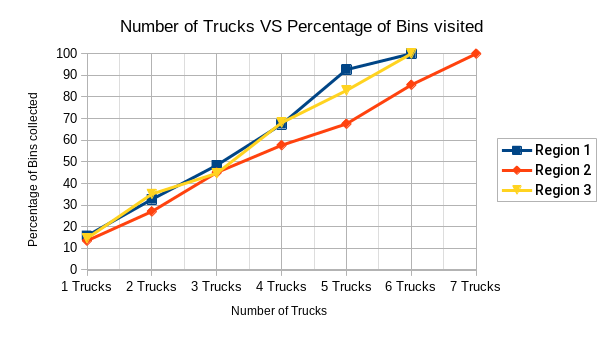
\includegraphics[width=\linewidth]{number_of_trucks_VS_bins_visited.png}
        \caption{Region-wise}\label{figc2}
    \end{subfigure}
    \caption{Effect of number of trucks on bin coverage}
    \label{fig3}
\end{figure}

 

\begin{figure}[H]
    \centering
    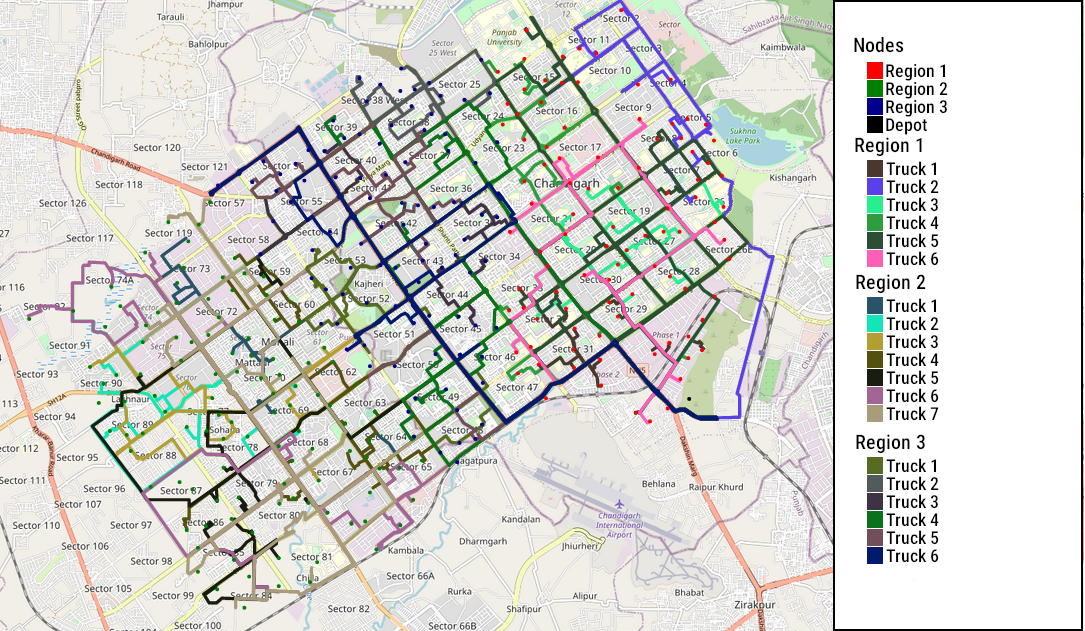
\includegraphics[scale=0.4]{Dynamic_weighted_unrestricted.png} % New Image added
    \caption{Realtime Unrestricted}\label{fig2}
\end{figure}


\subsubsection*{Case 3: Comparison of real-time with static route calculation}

Our base case of route calculation considers real time dynamics of waste (bin, truck) and truck's current position in real time. However, the existing collection system of the city is static. Hence, we compared the real-time route calculation model with static by modifying the eq \eqref{eq12} where the constraint will simply be less than 100, as shown in \eqref{eq12x}. In equation \eqref{eq2} and Eq \eqref{eq3}, instead of \textit{st}, the beginning nodes will always be 0 (\eqref{eq2x}\eqref{eq3x}). 
\begin{equation}\label{eq12x}
    u_i\le 100
\end{equation}
\begin{equation}\label{eq2x}
    \sum_{j\in N}X_{0,j}=1 ; \forall j \in N
\end{equation}
\begin{equation}\label{eq3x}
    \sum_{j\in N}X_{j,0}=1 ; \forall j \in N
\end{equation}

The above constraints when implemented results in a fixed optimal route which doesn't change with the time. We executed the dynamic and static models for 3 trucks per region, for a total of 9 trucks. The comparison is represented in Table \ref{tab5}

\begin{table}[H]
    \centering
    \caption{Comparison of static and real-time optimization performance} \label{tab5}
    \vspace*{0.3cm}
    \begin{tabular}{|c|c|c|c|}
        \hline Case & Waste (Kg) & Distance (Km) & Percent Covered\\
        \hline \textit{Static}& 8996.88 & 798.13 & 40.33\%\\
        \hline \textit{Real-Time}& 8967.25 & 517.8 & 46.00\%\\
        \hline
    \end{tabular}
\end{table}

The routes (Figure \ref{fig4} and Figure \ref{fig5}) show the routes obtained for static and dynamic case for 9 trucks. The outcomes demonstrate the consideration of dynamic variables on the routes which are different than the static model. 

\begin{figure}[H]
    \centering
    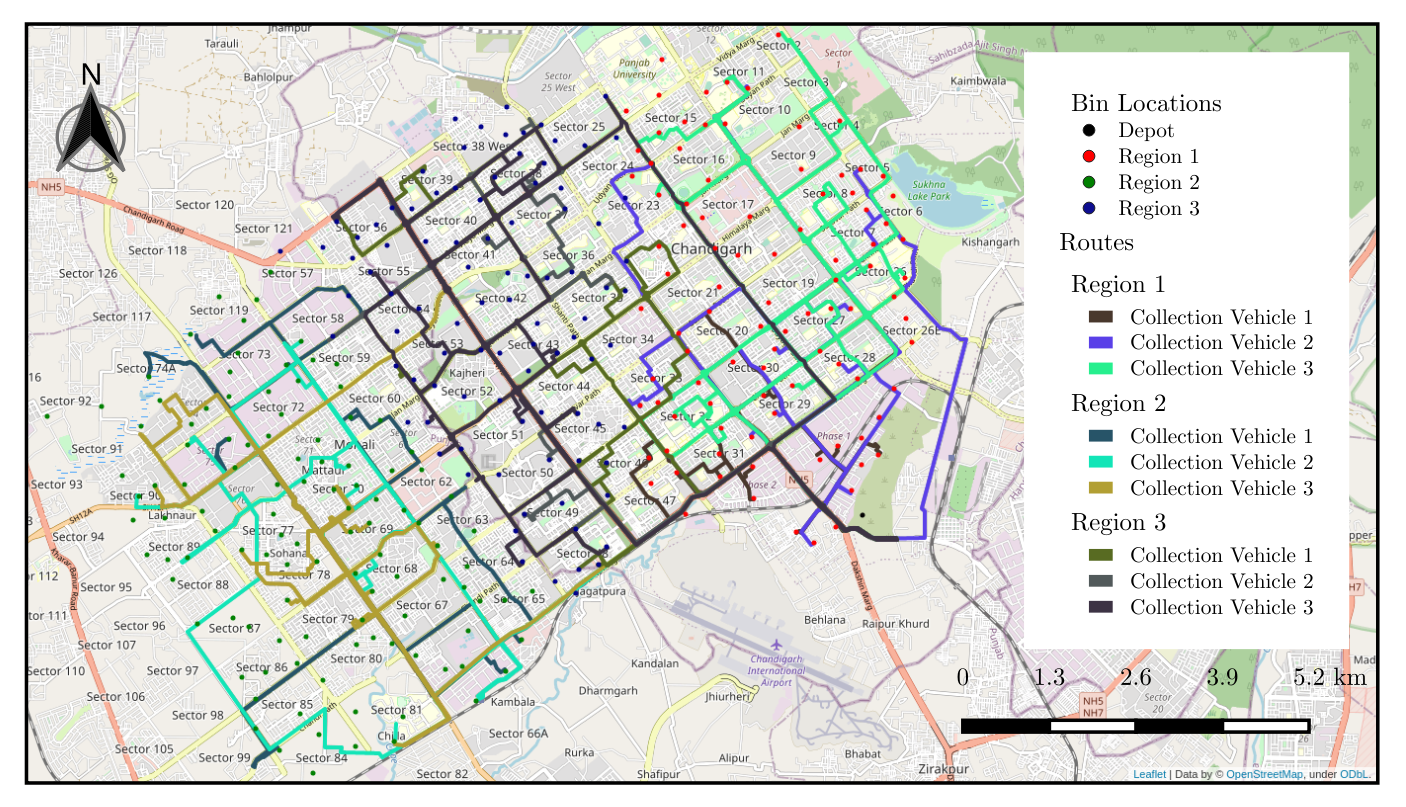
\includegraphics[scale=0.3]{Static_Weighted_3_Truck.png} % Image changed here
    \caption{Routes for 3 truck per region as calculated by static optimization}\label{fig4}
\end{figure}
\begin{figure}[H]
    \centering
    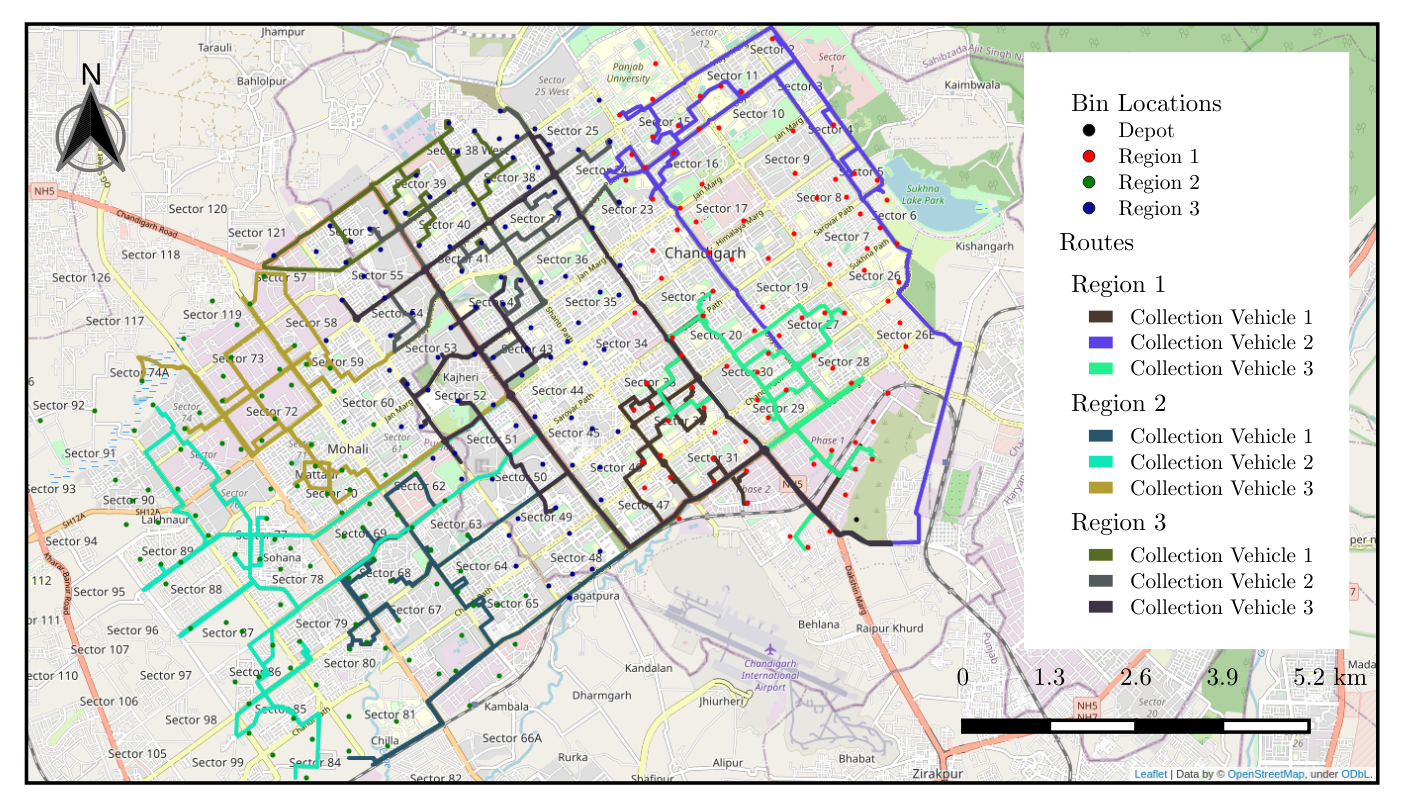
\includegraphics[scale=0.3]{Dynamic_weighted_3_Truck.png} % Image changed here
    \caption{Routes for 3 truck per region as calculated by real-time optimization}\label{fig5}
\end{figure}

\begin{figure}[H]
    \centering
    \begin{subfigure}{0.5\textwidth}
        \centering
        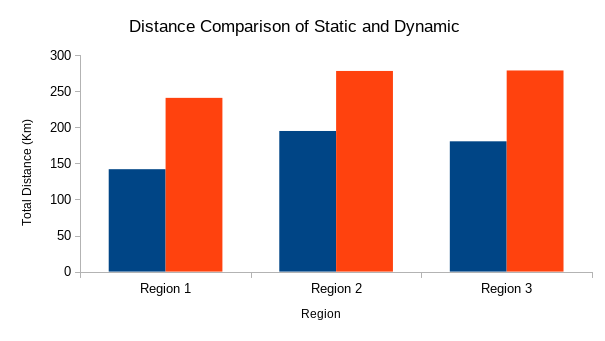
\includegraphics[width=\linewidth]{Total Distance Comparision of Static and Dynamic.png}
        \caption{Distance comparison}\label{figh1}
    \end{subfigure}%
    \begin{subfigure}{0.5\textwidth}
        \centering
        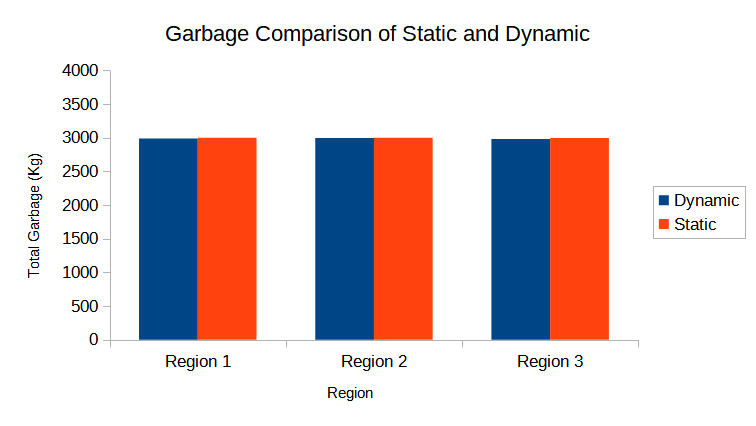
\includegraphics[width=\linewidth]{Total Garbage Comparision of Static and Dynamic.png}
        \caption{Waste comparison}\label{figh2}
    \end{subfigure}
    \caption{Comparison between static and real-time models}
    \label{figh}
\end{figure}

We used the case of 3 vehicles per region in order to achieve a suitable middle ground, providing enough complexity to the problem for the two models to be fully utilized and compared while also maintaining the resource constrained aspect of the problem. We observe that the weight of the waste collected is nearly the same for both cases but the distance travelled by the trucks in the real-time case is significantly less than the static case. This further emphasizes the efficiency of the real-time method over the static method.

This makes real-time optimization the superior model in terms of both efficiency and features. In the static model, there is no accounting for new data. The initial route is the only route that is calculated. This, consequently, also makes it unreliable. Real-time model, on the other hand, accounts for new data and creates new optimal routes taking it into consideration, making it very adaptable and robust. Since real-time is just a modified and iterated version of the static model, the difference in computational power required between the two methods is not large. 

Therefore, for real life applications, real-time model is the preferred method as it is able to deal with non-deterministic events that are synonymous with ground use and adapt to them, giving an uninterrupted and reliable service, while also providing greatly efficient results.


 
\subsubsection*{Sensitivity Analysis of Weights}
In order to depict the effect of selected objective function weights on the waste  (\ref{figs1})  collected and the distance travelled by the collection trucks (\ref{figs2}), we performed a detailed sensitivity analysis. The Figures indicate that weights had highly non linear influence on the total distance travelled collected than the garbage collected. We normalized the distance and garbage collected values for their comparison (see \ref{figs}). From the graph it can be observed that the weight combinations such as W1=0.9,W2=0.1; W1=0.4,W2=0.6 can be reasonably good for maximizing the collection of waste at minimum distance cost (W1=0.9,W2=0.1). The outcome is also inline with our selected weights. The analysis as a decision making tool can help  in selecting the best weights for desired scenarios.

\begin{figure}[H]
    \centering
    \begin{subfigure}{0.5\textwidth}
        \centering
        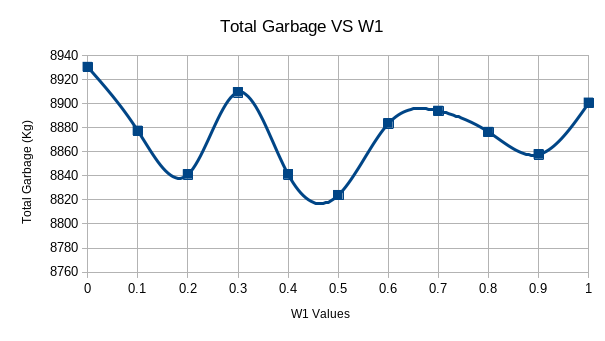
\includegraphics[width=\linewidth]{Total_Garbage_VS_W1_3_Trucks.png}
        \caption{Waste vs $w_1$}\label{figs1}
    \end{subfigure}%
    \begin{subfigure}{0.5\textwidth}
        \centering
        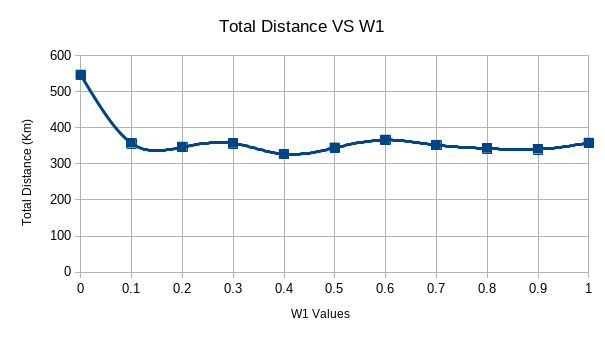
\includegraphics[width=\linewidth]{Total_Distance_VS_W1_3_Trucks.png}
        \caption{Distance vs $w_1$}\label{figs2}
    \end{subfigure}
    \caption{Effect of weight on waste and distance for 3 trucks per region}
    \label{figsz}
\end{figure}

\begin{figure}[H]
    \centering
    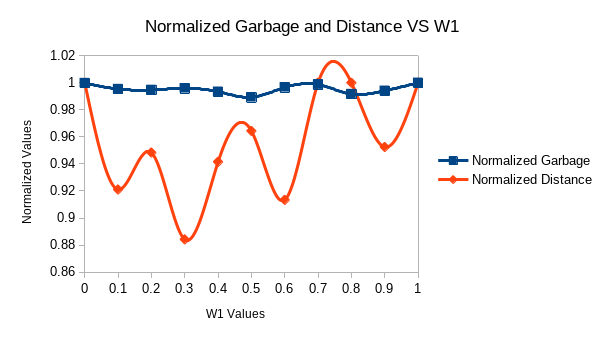
\includegraphics[scale=0.6]{Distance and Garbage Normalized VS W1.png}
    \caption{Normalized weight sensitivity graph}\label{figs}
\end{figure}

\textcolor{red}{One of the most noticeable observations that can be derived from the sensitivity analysis is the changes in the distance and waste as the weights are varied. The behaviour seems anomalous at first glance, but it can be explained by the fact that the weights do not directly affect the waste collected and distance travelled. The weights only directly affect the objective function and the new routes that are calculated by it, as a result, affect the distance and waste values. Therefore, as the weights are changed, the calculated routes change. Since the paths in real life are not continuous, that is, they do not have paths of every possible length, the distance travelled and similarly, the waste collected values vary significantly as the weights vary.} 

\textcolor{red}{However, we must keep in mind that this does not mean that the paths calculated are unideal. The calculated routes are still the best possible routes following all of the specified requirements and constraints.}




\section{Discussion}

The collection of waste is a highly visible and important municipal service that involves large expenditures. Waste collection problems are, however, one of the most difficult operational problems to solve, as it involves a lot of complex dynamic activities. Without modeling these activities a solution often have limited on-ground implementation. Our objective in this paper addresses these challenges by simultaneously modeling the dynamic changes in waste values of bin and truck to dynamically update the routes for maximizing the collected waste while covering less distance. Moreover, the consideration of dynamic bin values replicates the realistic scenario. A very few research has coupled such variations with the dynamically varying routes based on the model objective. The outcomes of various experiments prove that our methodology outperforms the existing static method of waste collection. Our model was able to collect almost similar amount of waste in significantly less travelled distance. This can have direct implications on the carbon footprint and eventually on developing sustainable societies.

Another important aspect of a sustainable system that this study addresses is strategic planning of the available resources. As a general theory a lot of resources can solve the problem. However, this can be a challenge for a resource constrained society, as the resources are limited and their availability may not be sufficient for the amount of waste generated. A way to address this can be using alternate methods such as multiple collection runs per vehicle. However, this will have time limitations and can also lead to subpar waste collection, considering the dynamics of wastes. The outcomes of the model execution show that using a reasonably less number of collection trucks a large area can be catered with good efficiency. Further, the performed sensitivity analysis of various objective weights as a decision making tool can help planners preempt the collection scenarios, which makes this system highly relevant to city managers.
Unlike the currently implemented systems with limited dynamic considerations, our solution:
\begin{itemize}
   
    \item is capable of calculating optimal paths based on the dynamic updates (real-time fill levels of smart bins, priority to bins based on fill values, vehicle position and its fill levels ) that generally happen in real-time.
    \item significantly improves the performance of waste collection system in terms of distance travelled and waste collected.
    \item reduces the distance overheads by removing the need to visit redundant nodes.
    \item being generic can be implemented to any city across the globe by updating the specific objectives and constraints. 
    
    \item addresses the challenges of decision makers concerning a system that could be implemented in the realistic environment. Our approach of modeling the problem as linear programming model makes it ideal for integrating it with a real-time system. 

\end{itemize}

The paper put forwards following major policy suggestions that can be implemented to to support the vision of creating smart sustainable cities:

\begin{itemize}
\item Inclusion of waste collection system in climate resilience plan: Climate resilience based urban planning is at the centre of major decision-making systems. Waste collection involves trips of collection vehicles, which adds to carbon emission. Strategic routing of available vehicles can not only benefit the economic aspects but can also help reduce the carbon emissions. To achieve this the government can include the waste collection system with the climate resilience plan of the city. The methodology proposed in this research can serve as an important component of such systems.
    
\item Implementation of smart bins for community or regions:  Door-to-door collection of waste is not practiced in majority of city/town. The issue is even more challenging in dense urban regions with narrow lanes where accessibility of vehicles can be limited. However, smart bins for various unorganised and organized built-up regions can address the challenge. Smart bins with sensors that send fill details can help in prioritising them leading to better collection and routing strategies on the similar lines to our method. The information of waste type automatically sensed using smart sensors can further benefit the waste segregation which is an another major challenge in waste management.\cite{actionplan}

 \item On-board computation: Future smart cities are going to be developed using modern technologies as its backbone. Technology can immensely benefit waste collection by implementing  numerous technologies in everyday collection practices. One of these valuable pieces of equipment is the on-board computation. The routing module proposed in the study integrated with Global Navigation Satellite Systems (GNSS) can be implemented in on-board computer for generating routes . Not only can the driver follow his route on the system, but can also communicate with the office notifying them of any important information. Benefits that increase driver efficiency are:
 \begin{itemize}
 \item Track routes in real-time
   \begin{itemize}
 \item relief driver can run route without any prior knowledge of it,  which can reduce unnecessary time and cost.\item the generated trip data can further be used to update the routing model based on the future requirements.
   \item brings accountability to the system as stakeholders (decision makers, citizen) can track the vehicle and plan accordingly. Moreover, the decision makers can quantify the effectiveness of the collection process. 
    
 \end{itemize}
 \item Integration with billing systems with smart bins
   \begin{itemize}
 \item by integrating the billing system in the routing software with smart bins, customers can for charged for extra collection thus not missing additional revenue. \item customers can also be charged for not segregating waste at the collection point, which can address the segregation process challenges, and will help bring accountability in the system.
\end{itemize}
\end{itemize}
\end{itemize}
\section{Conclusion}
\textcolor{red}{There has been a noticeable lack of work in real-time optimization of VRP compared to standard static optimization. This paper fills that gap by designing a flexible real-time route optimization model that accepts and adapts to constantly updating data to provide optimal routes. This makes the model excellent for real world applications as it can take care of unseen circumstances and automatically adapt to them with little modification. The routes formed by real-time optimization have also been shown to be much more efficient when compared to static optimization models, reducing the distance travelled by around 35\% for the same amount of waste collected (Table \ref{tab5}).}

\textcolor{red}{The paper also fills the relatively niche research gap of VRP applications in resource constrained societies and developing countries. It achieves that goal by creating and testing the model for the city of Chandigarh, India. Chandigarh, being a relatively well planned city, still has many unplanned regions, This allowed us to test the effects of our model for both a developing as well as developed city. This enabled the model to deal with the challenges of a resource constrained society, while also being able to be scaled for a developed region. The paper also focuses on the policy application side of this problem. The sensitivity analysis allows decision makers to decide on the best compromise that is possible for limited resources and the unrestricted case details the minimum amount of resources that are needed to cover the whole region.}

Scopes for future development may focus on improving upon our works by integrating more detailed street data like street signs, one-way roads and using the additional parameters as factors to provide a more street accurate route tailored for a specific region. Further integration of real time data such as accidents, construction work etc. in route calculations to provide a more robust and exception friendly model may also be considered for further works.

Future forays into this field may also focus on the effects different sets of weights may have on the results of the objective function for more granular levels of resource constraint. In our current work, we have focused solely on the best weights for one specific case and sensitivity analysis for resource constrained case. So further research can be done to find a more concrete relationship between weights, results and resource availability. In our current method of real time route calculation, our algorithm does not consider the route already travelled when calculating the new routes for new data. This leads to some degree of inefficiency in the optimization process and is also a viable topic for further work in this field.
\bibliographystyle{ieeetr}

\bibliography{citation}
\end{document}